O \textit{benchmark} bench4Q define uma carga de trabalho, incluindo banco de dados, transações, regras de execução e de taxa de transferência e métricas de resposta.  Para expor a dinâmica de um sistema é necessário estimulá-lo através da carga de trabalho, que é o componente responsável por estimular o sistema através de cenários ou fenômenos de \textit{burstiness}. Essa implementação é composta por classes e métodos, esse conjunto de código é um componente básico do \textit{benchmark} que refere-se a uma unidade de trabalho genérico que envia a carga para o sistema. O \textit{burstiness} incluem solicitações HTTP, chamadas de procedimento remoto, invocações de serviços Web, transações de banco de dados, comandos interativos ou também mesmo poderia ser composto de múltiplas tarefas de processamento, por exemplo sessões de cliente que compreendem várias solicitações ao sistema, etc \cite{Kounev2005}. Segundo \cite{Nobile2013} uma alteração na entrada (carga de trabalho) fará com que o sistema saia do estado de regime estacionário e entre em um período de regime transiente que descreve a dinâmica de um sistema, o regime transiente é calculado para uma entrada degrau unitário.

O objetivo deste trabalho é estender a carga de trabalho do \textit{benchmark} de tal maneira que permite-se estimular o sistemas a apresentar a sua dinâmica, assim possibilitando a analise transiente do sistema. 

Conforme apresentado no capitulo \ref{chapter:revisao}, o \textit{benchmark} Bench4Q oferece uma interface gráfica para configuração e colete dos dados, o que facilita a sua operação e analise. A proposta da extensão deste trabalho é possibilitar a modulação da carga, também, via interface gráfica, onde será necessário o preenchimento alguns conjuntos de parâmetros para a geração da carga.

\cite{Binnig2009} os serviços em nuvem de hoje diferem entre outros pelo custo, desempenho, garantias de consistência, balanceamento de carga, \textit{caching}, tolerância a falhas, SLA e linguagem de programação. Para a discussão deste trabalho, assumimos um sistema de \textit{n-tiers} que consiste nos seguintes componentes:

\begin{itemize}
	\item \textbf{Gerador de Carga (\textit{Workload}) :}
	\item \textbf{Balanceador de carga (\textit{Load Balancer}):}
	\item \textbf{Servidor Físico (\textit{Hypervisor}):}
	\item \textbf{Servidor de dados (\textit{Data base}):}
\end{itemize}

Para o desenvolvimento deste trabalho, assumimos uma arquitetura composto conforme a figura\ref{fig:arquitetura-experimento}.

\begin{figure}[!htb]
	\centering
	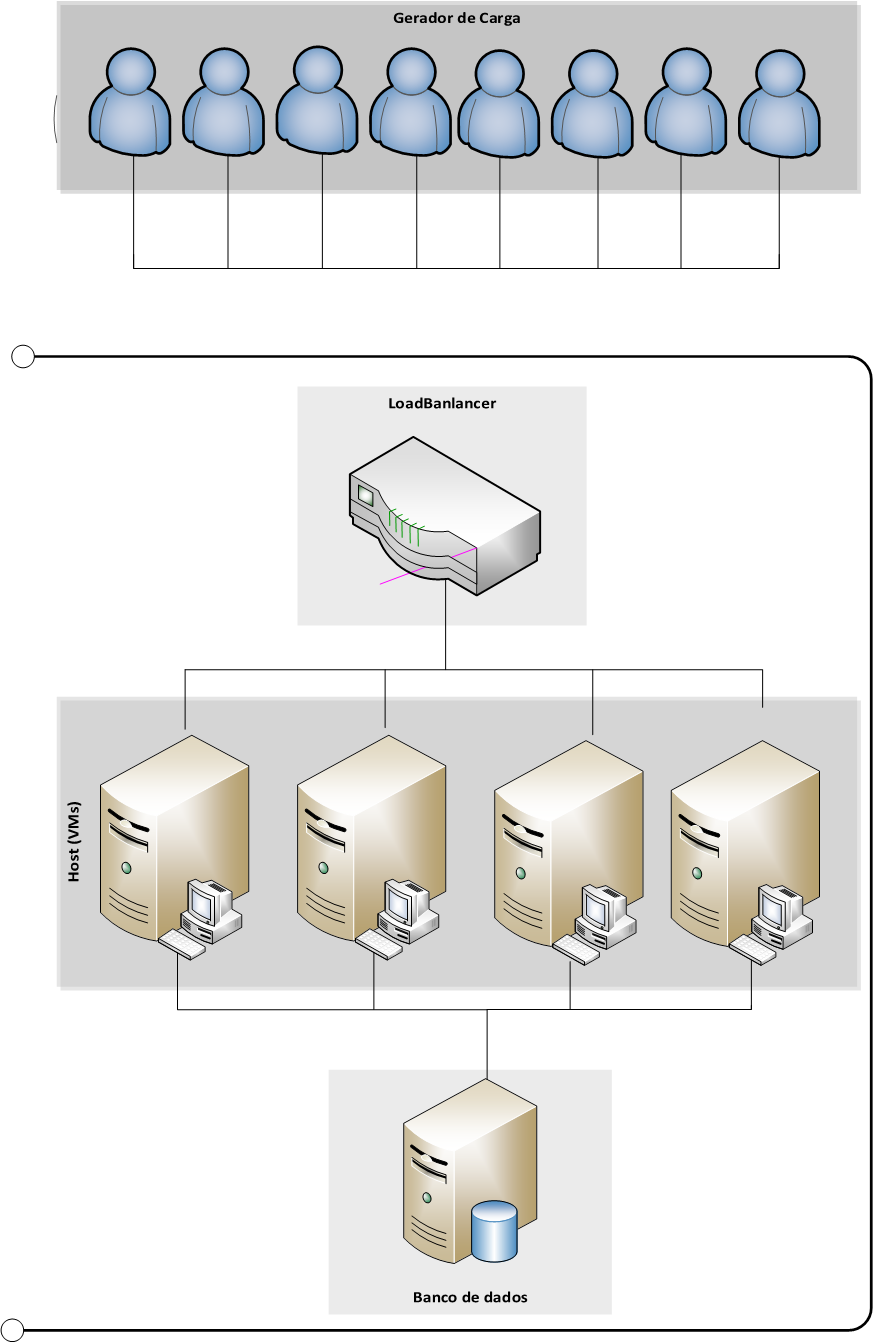
\includegraphics[scale=0.55]{arquitetura-experimento.png}
	\caption{Arquitetura do experimento}
	\label{fig:arquitetura-experimento}
	\fautor
\end{figure}


O ambiente utilizado para execução dos experimentos é apresentado na Tabela \ref{tab:configuracao_maquinas}.
Foram utilizadas oito unidades para a geração de carga (\textit{workload}) que atuam como clientes dos serviços, uma unidade de balanceamento de carga e 4 servidores atuando como provedor de serviços e uma unidade executando o banco de dados a ser consultado pelo provedor de serviços.

\begin{table}[htb]
	\centering
	\caption{Especificação do ambiente de execução dos experimentos}
	\label{tab:configuracao_maquinas}
	\begin{tabularx}{\textwidth}{|r|c|X|} \hline\hline
		\textbf{Componente}    & \textbf{Quantidade} & \textbf{Configuração} \\ \hline
		\textit{Workload}      & 8 Unidades          & Intel Core 2 Quad Q6600 2.4GHz, 4GB de RAM \\
		\textit{Load Balancer} & 1 Unidade           & Intel Core 2 Quad Q6600 2.4GHz, 4GB de RAM \\
		\textit{Hosts}         & 4 Unidade           & Intel Core 2 Quad Q6600 2.4GHz, 4GB de RAM \\
		\textit{Data base}     & 1 Unidade           & Intel Core 2 Quad Q6600 2.4GHz, 4GB de RAM \\
		\hline
	\end{tabularx}
	\fdadospesquisa
\end{table}

Neste trabalho vamos nos concentrar na modulação correta da carga de trabalho, assim.a carga de abranger os seguintes cenários:
\begin{itemize}
	\item \textbf{tempo de sobrecarga planejada:} Um período de tempo em que a carga de trabalho é máxima, caracterizado o crescimento de requisições inesperada,
	\item \textbf{tipo de modulação:}
	\item \textbf{quantidade de agentes da sobrecarga:}
\end{itemize}


A metodologia de extensão descreve as etapas necessárias para as modificações, a presente metodologia permite que se obtenha uma carga de trabalho que estimule o sistemas a apresentar a sua dinâmica, assim possibilita a analise transiente do sistema. De acordo com \cite{KaiSachs2010}, uma metodologia de desenvolvimento de \textit{benchmarks} deve incluir em seu processo de desenvolvimento, bem como a sua execução e a análise dos seus resultados. Para tanto é necessário medir o comportamento do sistema com a base me métricas. A métrica é uma função que transforma resultados medidos em uma forma facilmente compreendida. \cite{Folkerts2013} As métricas de referência deve permitir caracterizar e quantificar o comportamento do sistema quando enfrenta perturbações (ou seja, falhas, ataques, e variações de ambiente operacional) \cite{Marco2012}. As métricas tradicionais, de analise estacionaria, não podem capturar os comportamentos transitórios do sistema em resposta às variações de carga implementada no primeiro passo dessa metodologia.

No contexto de avaliação transiente, \cite{Rosu1997} afirma que a reatividade da métrica é muitas vezes mais importante do que a otimização da mesma, no mesmo trabalho, \cite{Rosu1997} apresenta a característica e comportamento de uma métrica transiente, conforme ilustrado pela figura \ref{fig:transient-metric}, que são: 
\begin{itemize}
	\item \textbf{\textit{Reaction Time} (Tempo de reação)} - o período entre a ocorrência da variação crítica e a conclusão da promulgação realocação de correção;
	
	\item \textbf{\textit{Recovery Time} (Tempo de Recuperação)}  - o intervalo entre a conclusão promulgação e da restauração de um nível de desempenho aceitável;
	
	\item \textbf{\textit{Performance Laxity} (Frouxidão performance)} - a diferença entre o required v performance, e o desempenho em estado estacionário, após a redistribuição;
\end{itemize}


\begin{figure}[!htb]
	\centering
	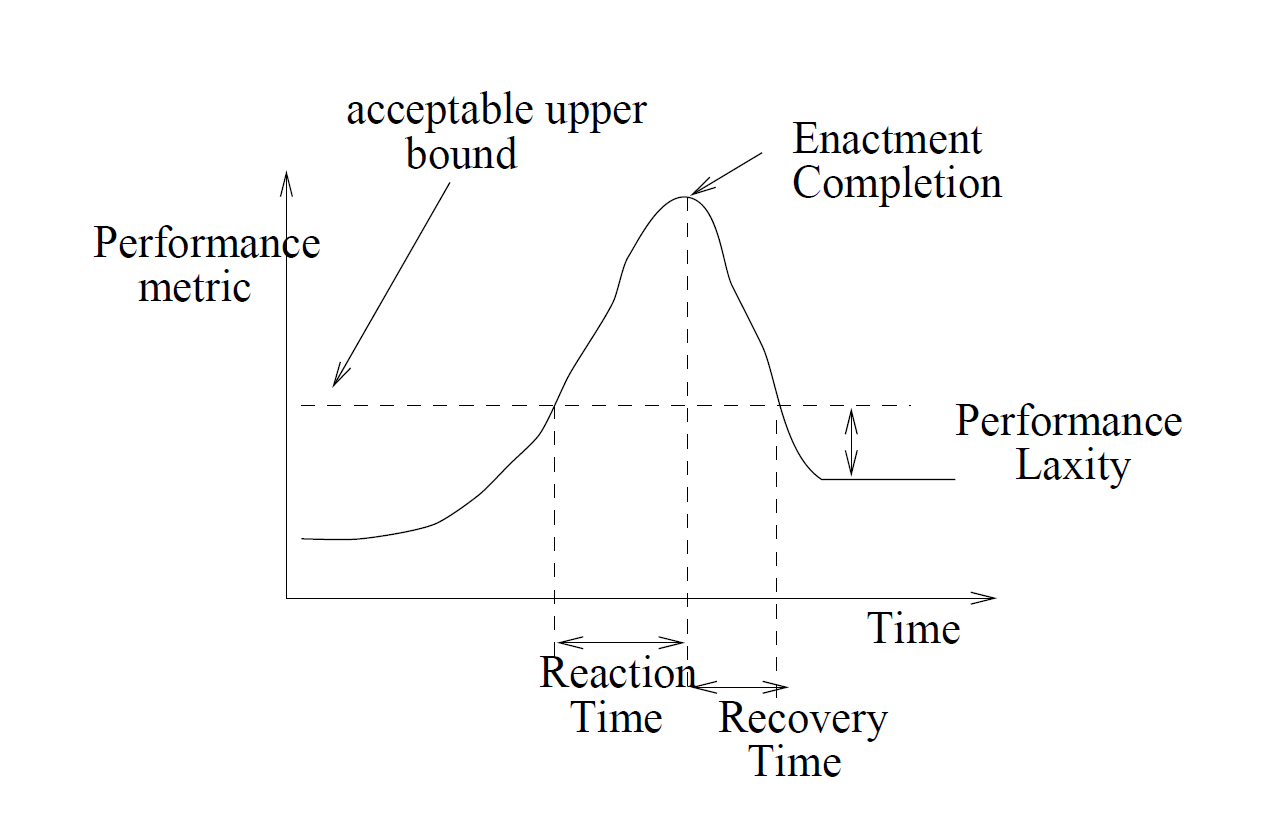
\includegraphics[scale=0.4]{transient-metric.png}
	\caption{Comportamento de métrica transiente}
	\label{fig:transient-metric}
	\fdireta{Rosu1997}		
\end{figure}


A métrica em questão deve ser identifica dentro da realidade e necessidade em que se encontra o sistemas a ser avaliado. Logo será de uma ingenuidade fixar uma métrica para um sistema desconhecido, o importante é que ela tenha o comportamento e as características apresentadas anteriormente nesse passo da metodologia de extensão. Existem diversos trabalhos dedicados que identificam métricas transiente em vários contextos como o \cite{Binnig2009, Lu2000, Rosu1997}.

\cite{Binnig2009} afirma que os \textit{benchmarks} tradicionais são principalmente preocupados com o desempenho e o custo de sistemas estáticos e essas métricas ainda tem relevância para as aplicações em nuvem, mas é necessário medir diferentes métricas para sistemas escaláveis (ou seja, dinâmico) onde os recursos vêm e vão. Ainda \cite{Binnig2009} enfatiza que os novos \textit{benchmarks} devem relatar métricas diferentes do que os benchmarks existentes: 
\begin{citacao}
	Em vez de medir o desempenho médio de um sistema estático em carga máxima, as novas métricas devem refletir a capacidade dos serviços em nuvem para se adaptar a uma mudança de carga com relação ao desempenho e custos. Além disso, uma métrica adicional também deve cobrir a robustez desses serviços contra falhas de nós individuais.
\end{citacao}

As métricas definidas precisam refletir o cenários de dinâmica do sistema, que inclui três aspectos principais:
\begin{itemize}
	\item \textbf{Conexões por segundo (Load Balancer):} Conforme sugerido por \cite{Binnig2009}, medir a escalabilidade através do aumento dos interações web emitidos por segundo ao longo do tempo e de forma contínua contando o interação web que são respondidas em um intervalo de tempo de resposta.
	\item \textbf{Tempo de resposta (\textit{browsers}):}
	\item \textbf{Consumo de CPU (VMs):}
	\item \textbf{Alguma na base de dados}
\end{itemize}
%• custo de capital: O custo de hardware e software adicional necessário para um sistema de HA em comparação com um sistema não-HA outra forma equivalente.
%• impacto Performance: O impacto para o desempenho de recursos de alta disponibilidade durante as operações normais em comparação com o sistema de não-HA.
%• Tempo de recuperação: O tempo para restaurar o serviço de banco de dados após a ocorrência de uma falha.


Os experimentos conduzidos neste trabalho consideraram três diferentes fatores de dois níveis cada, conforme aprestando na Tabela \ref{tab:fatores_niveis}. 

\begin{table}[htb]
	\centering
	\caption{Fatores e níveis dos experimentos}
	\label{tab:fatores_niveis}
	\begin{tabularx}{\textwidth}{|c|c|c|c|} \hline\hline
		Fatores  & \textit{Workload} & Banco de dados & Politica de Alocação de recursos\\ \hline
		Nível 1  &         			 & Postgres 	  & Estática                        \\
		Nível 2  &            		 & DB2 			  & Dinâmica                        \\
		\hline
	\end{tabularx}
	\fdadospesquisa
\end{table}


O primeiro fator refere-se à quantidade de clientes simultâneos requisitando serviços ao Serviço Web, esses clientes são modulados conforme a configuração feita, sendo assim essa carga de trabalha estimulará o sistema a apresentar a sua dinâmica. O segundo fator associado a possibilidade de serem considerados diferentes tipos de serviço, assim este fator terá dois níveis de bancos de dados o Postgres e o DB2, o Bench4Q oferece o \textit{script} de criação de bando para ambos. O último e o terceiro fator, se refere a política de alocação de recursos, neste caso são dois níveis \textit{estática} (onde os servidores \textit{host} estão desde o princípio em execução e disponíveis.) e \textit{dinâmica} (onde os servidores são colocados à disposição conforme a oscilação da carga de trabalho).

O planejamento de experimento e utilizado neste trabalho como avaliação de desempenho segue a abordagem do planejamento fatorial completo. Logo, possibilita que todas as combinações possíveis dos fatores sejam examinados. Para cada experimento serão 5 repetições, utilizadas para determinar a média, o desvio padrão e o intervalo de confiança de 95% .

Durante a execução dos experimentos pequenas aplicações, monitores, em cada um dos níveis da arquitetura são responsáveis por coletar algumas informações de interesse disponíveis, como a taxa de utilização de CPU e a quantidade de requisições simultâneas. Os valores produzidos pela experimentação foram adicionados em arquivos Excel (\textit{.xls}), esses dados foram processados pelo R \footnote{\url{https://www.r-project.org/}}.
